\section{Régression linéaire avec plusieurs variables}
\subsection{Normalisation des caractéristiques}

Dans ce problèmes nous avons des caractéristiques qui ont des échelles radicallement différentes \textit{(exemple 2100 sq-ft pour 3 chambres)}. Il est intéressant de normaliser c'est données pour les ramener à une échelle comune, 
ce qui permet d'interpréter plus facilement les résultat et rendre les calculs plus stable et rapide. Grâce à la normalisation on peut être sûr que chaque caractéristiques contribue équitablement à la prédiction du modèle, indépendamment de son échelle initiale. \\

\noindent
Pour réaliser la normalisation nous pouvons établire les formules suivantes:

\begin{figure}[!h]
    \centering
    \begin{minipage}{.33\linewidth}
        \begin{equation*}
            X_{norm} = \frac{X - \mu}{\sigma}
        \end{equation*}
    \end{minipage}\hfill\vline
    \begin{minipage}{.33\linewidth}
        \begin{equation*}
            \mu = \frac{1}{m} \sum_{i=0}^{m-1}x_j^{(i)}
        \end{equation*}        
    \end{minipage}\hfill\vline
    \begin{minipage}{.33\linewidth}
        \begin{equation*}
            \sigma = \sqrt{\frac{1}{m} \sum_{i=1}^{m} \left(x_j^{(i)} - \mu\right)^2}
        \end{equation*}                
    \end{minipage}
\end{figure}

\begin{itemize}
    \item $\mu$ La moyenne de chaques caractéristiques
    \item $\sigma$ L'écart type de chaques caractéristiques
    \item $X_{norm}$ Caractéristiques normalisées
    \item $x_j^{(i)}$ La caractéristique de la ligne $j$ à la colonne $i$
\end{itemize}

\clearpage

\vspace{.5cm}
\noindent
\textbf{Mise en application}
\vspace{.2cm}


\begin{figure}[!h]
    \begin{minipage}{.48\linewidth}
\begin{minted}[frame=lines, framesep=2mm, baselinestretch=1.2, fontsize=\footnotesize, linenos, breaklines=true]{python}
def featureNormalize(X):
    mu = np.mean(X, axis=0)
    sigma = np.std(X, axis=0)
    X_norm = (X - mu) / sigma

    return X_norm, mu, sigma
\end{minted}   
\captionof{listing}{Fonction featureNormalize}
    \end{minipage}\hfill
    \begin{minipage}{.48\linewidth}
        \begin{equation*}
            \begin{aligned}
                \mu &= [2000.68085106 \quad 3.17021277] \\
                \sigma &= [7.86202619e+02 \quad 7.52842809e-01]
            \end{aligned}
        \end{equation*}  
    \end{minipage}
\end{figure}


\subsection{Descente de gradient}

La descente de gradient de ce second problème, suit la même méthodologie. La seule différence est qu'ici on à plusieurs caractéristiques. \\
Nos fonction précédentes sont adapté pour un calcul de coût et une descente de gradient à plusieurs caractéristiques, nous pouvons réutiliser les mêmes fonctions.

\begin{figure}[!h]
\begin{minted}[frame=lines, framesep=2mm, baselinestretch=1.2, fontsize=\footnotesize, linenos, breaklines=true]{python}
def computeCostMulti(X, y, theta):  
   m = y.size
   J = 0

   for i in range(0, m):
      J += (1/(2*m)) * (X[i].T @ theta - y[i])**2
   
   return J
\end{minted}   
\captionof{listing}{Fonction computeCostMulti}\label{listing:computeCostMulti}
\end{figure}


\begin{figure}[!h]
\begin{minted}[frame=lines, framesep=2mm, baselinestretch=1.2, fontsize=\footnotesize, linenos, breaklines=true]{python}
def gradientDescentMulti(X, y, theta, alpha, num_iters):  
    m = y.size  # number of training examples
    n = theta.size # number of parameters
    cost_history = np.zeros(num_iters)
    theta_history = np.zeros((n,num_iters))

    for n_iter in range(num_iters):
        for j in range(n):
            res = 0
            for i in range(m):
                res += (X[i].T @ theta - y[i]) * X[i][j]
            
            theta[j] = theta[j] - alpha * (1/m) * res

        cost_history[n_iter] = computeCostMulti(X, y, theta)
        theta_history[:,n_iter] = theta.reshape((n,))
              
    return theta, cost_history, theta_history
\end{minted}   
\captionof{listing}{Fonction gradientDescentMulti}\label{listing:gradientDescentMulti}
\end{figure}


Suite à notre descente de gradient, on constate sur la figure \ref{fig:fig4} que le coût $J(\theta)$ converge vers un minimum. On peut donc considérer que nos valeurs de $\theta$ sont optimal pour réaliser une prédiction proche de la réalité.

\begin{figure}[!h]
    \begin{minipage}{.48\linewidth}
        \begin{center}
            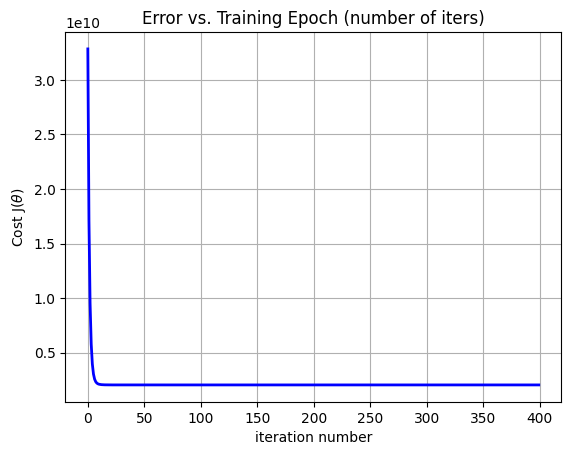
\includegraphics[width=1\textwidth]{./img/5-2.png}
            \caption{\label{fig:fig4}Convergence de $J(\theta)$ en fonction des itérations avec $\alpha = 0.3$}  
        \end{center}
    \end{minipage}\hfill
    \begin{minipage}{.48\linewidth}
        \begin{equation*}
            \begin{aligned}
                \theta_0 &= 340412.65957447 \\
                \theta_1 &= 109447.79 \\
                \theta_2 &= -6578.35
            \end{aligned}
        \end{equation*}  

        Prédiction pour une maison de 1650 \textit{sq-ft} et 3 chambres de 293081.46\$
    \end{minipage}
\end{figure}

\subsubsection{Sélection du taux d'apprentissage}

Comme expliqué précédement il est important de séléctionner correctement le taux d'apprentissage, si celui-ci est trop important alors la descente de gradient peut divergé d'un minimum, si il est trop petit alors le processus peut échouer dû à des 
valeurs trop importantes.

\vspace{.5cm}
\noindent
\textbf{Trop petit, $\alpha = 0.001$}
\vspace{.2cm}

\begin{figure}[!h]
    \begin{minipage}{.48\linewidth}
        \begin{center}
            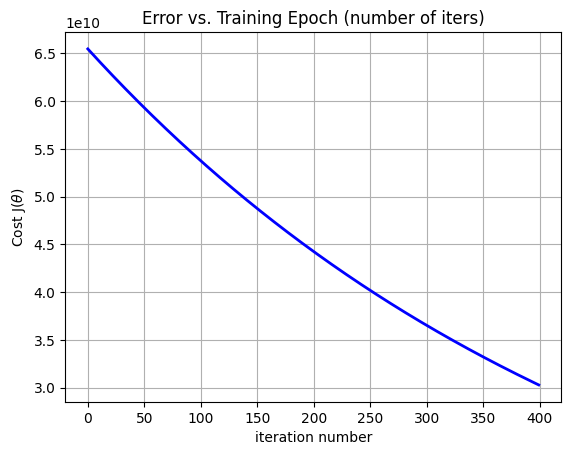
\includegraphics[width=1\textwidth]{./img/lowlearningrateng.png}
            \caption{\label{fig:fig5}Convergence de $J(\theta)$ en fonction des itérations avec $\alpha = 0.001$}  
        \end{center}
    \end{minipage}\hfill
    \begin{minipage}{.48\linewidth}
        \begin{equation*}
            \begin{aligned}
                \theta_0 &= 112272.89 \\
                \theta_1 &= 33255.72 \\
                \theta_2 &= 14509.19
            \end{aligned}
        \end{equation*}  

        Prédiction pour une maison de 1650 \textit{sq-ft} et 3 chambres de $94158.94$\$
    \end{minipage}
\end{figure}


Dans ce cas le taux d'apprentissage choisis est trop faible, on le constate grâce à l'allure de la courbe mais également avec les résultats obtenus. Un résultat cohérent se rapproche de l'allure de la figure \ref{fig:fig4}.

\subsection{Exercice facultatif: Equations normales}

La régression linéaire par équations normales donne un résultat similaire à la descente de gradient, mais ce n'est pas un algorithme itératif. L'équation \ref{eq:eq_normal} nous permet d'obtenir directement une 
valeur optimal de $\theta$.

\begin{equation}\label{eq:eq_normal}
    \theta = (X^T X)^{-1} X^T y
\end{equation}  


\vspace{.5cm}
\noindent
\textbf{Mise en application}
\vspace{.2cm}


\begin{figure}[!h]
    \begin{minipage}{.48\linewidth}
\begin{minted}[frame=lines, framesep=2mm, baselinestretch=1.2, fontsize=\footnotesize, linenos, breaklines=true]{python}
def normalEqn(X,y):
    theta = np.linalg.inv((X.T @ X)) @ X.T @ y

    return theta
\end{minted}   
\captionof{listing}{Fonction normalEqn}\label{listing:normalEqn}
    \end{minipage}\hfill
    \begin{minipage}{.48\linewidth}
        Prédiction pour une maison de 1650 \textit{sq-ft} et 3 chambres de $293081.46$\$ avec la méthode des équations normal. \\
        Le résultat est similaire de celui obtenus par la méthode de la descente de gradient avec une valeur de $\alpha = 0.3$.
    \end{minipage}
\end{figure}
